% v1.7 - 2014-01-07
% - font color changed
% - titlepage changed
% v1.6 - 2013-05-13

\documentclass[twoside,11pt,titlepage,a4paper,english,bibliography=totocnumbered,listof=numbered]{scrbook}

% Template Style
% =========================================================================
% = EduTec THESIS/PROJECT TEMPLATE STYLE
% =========================================================================


% ------------------------
% 


% =========================================================================
% = CHANGELOG
% =========================================================================

% [0.1.5]
% different colors
% new footer
%
% [0.1.4a]
% title page: image logo sizes and margins adjusted to printable area
% removed separation of online and offline references
%
% [0.1.3]
% wider text body
% added "school" to the titlepage
% paragraph indents
% correctly placed footnote graphics
% 
% [0.1.2]
% new titlepage
% some minor fixes
% 
% [0.1.1]
% changed titlepage logo
% added listoffigures and listoftables
% excluded abstract from toc
% no (roman) numbering for frontmatter
% 



% =========================================================================
% = MISC
% =========================================================================

\usepackage{a4wide}					% 
\usepackage{verbatim}				% 
\usepackage[toc,page]{appendix}			% 
\usepackage[withpage]{acronym}			% 
\usepackage{amsthm}				% Definitions


% =========================================================================
% = COLORS
% =========================================================================

\usepackage{xcolor}					% Colors
\definecolor{LightBlue}{rgb}{0.25,0.5,0.72}
\definecolor{DarkBlue}{rgb}{0,0.33,0.62}

% =========================================================================
% = PAGE LAYOUT
% =========================================================================

\usepackage{geometry}
\geometry{inner=3cm, outer=2cm, bottom=4cm}

\newcommand{\setwidesite}				% changes the geometry to have less margin
{
	\fancyhfoffset[LE,RO]{0cm}
	\fancyheadoffset[LO,RE]{0cm}
	\fancyfootoffset[RE]{2cm}
	\newgeometry{inner=2cm, outer=2cm, bottom=4cm}
}

\usepackage{noindent}				%do not indent at new paragraphs but add a vertical offset

\setlength{\parindent}{4mm}
\setlength{\parskip}{1.5mm }


% =========================================================================
% = TYPESETTING
% =========================================================================

\usepackage[hyphens]{url}				% url
\usepackage{hyphenat}				% hyphenation. use \hyphenation{}

\righthyphenmin=5
\lefthyphenmin=5


% =========================================================================
% = TABLE OF CONTENTS
% =========================================================================

\setcounter{secnumdepth}{4}
\setcounter{tocdepth}{3} 


% =========================================================================
% = FONTS
% =========================================================================

%\usepackage{mathpazo} 
%\usepackage[scaled=.95]{helvet} 
%\usepackage{courier} 
\usepackage{helvet}
\renewcommand{\familydefault}{\sfdefault}
\fontfamily{phv}\selectfont

% =========================================================================
% = SYMBOLS
% =========================================================================

%\usepackage{gensymb}
\usepackage{textcomp} 				% for \textmu (non-italic $\mu$)
\makeatletter						% this makes "@" a regular letter


% =========================================================================
% = TABLES
% =========================================================================

\usepackage{tabularx}
\usepackage{booktabs}
\usepackage{multirow}
\usepackage{longtable}				% tables spanning over more than one page

%%\setlength{\fboxsep}{0mm}			% spacing between \fbox border and content

\usepackage{amsmath}				% math fonts
\usepackage{amssymb}				% math symbols
\usepackage{setspace}				% line spacing 


% =========================================================================
% = BIBIOGRAPHY
% =========================================================================

\usepackage[style=numeric,backend=bibtex]{biblatex}

% apparently no effect?
%\renewcommand{\bibsetup}{
%	\markboth{
%		\MakeUppercase{Bibliography}
%	}{}
%}

\ifdefined\bibheadingonline
  \defbibheading{online}{\section*{\bibheadingonline}}
\else
  \defbibheading{online}{\section*{Online References}}
\fi
\ifdefined\bibheadingoffline
  \defbibheading{offline}{\section*{\bibheadingoffline}}
\else
  \defbibheading{offline}{\section*{Printed References}}
\fi

\defbibfilter{online}{%
  \( \type{online} \)}

\defbibfilter{offline}{%
  \( \not \type{online} \)}

\bibliography{main}


% =========================================================================
% = LANGUAGE & ENCODING
% =========================================================================

\usepackage[english]{babel}				% \usepackage[ngerman]{babel}

\selectlanguage{english}				% \selectlanguage{ngerman}

\usepackage[T1]{fontenc}
\usepackage[utf8]{inputenc}				% can use native umlauts

% \usepackage[babel,german=quotes]{csquotes}	% provides \enquote{Blupp} => "`Blupp"'
\usepackage[babel,english=american]{csquotes}	% provides \enquote{Blupp} => "`Blupp"'

\SetCiteCommand{\parencite}			% Changed for biblatex

\usepackage{units}					% unified way of setting values with units

\usepackage{appendix}


% =========================================================================
% = CODE LISTINGS
% =========================================================================

\usepackage{listings}

% Listings Styles from Max 

\definecolor{violet}{cmyk}{0.45,0.97,0.27,0.21}
\definecolor{lstblue}{cmyk}{1,0.80,0,0}
\definecolor{lstgreen}{cmyk}{0.71,0.21,0.65,0.22}
\definecolor{bluegrey}{cmyk}{0.56,0.24,0.11,0.05}
\definecolor{javadoc}{cmyk}{0.88,0.59,0,0}
\definecolor{lstgrey}{cmyk}{0.55,0.44,0.42,0.32}

\lstdefinelanguage{SQL}{
     keywords={},
     keywordstyle=\color{bluegrey}\bfseries,
     morekeywords=[2]{CREATE,TABLE,IF,NOT,EXISTS,NULL,SET,DEFAULT,PRIMARY,KEY,COLLATE,CHARACTER,AUTO_INCREMENT,ENGINE,CHARSET},
     keywordstyle={[2]\color{violet}\bfseries},
     otherkeywords={int,varchar,double,text,tinyint},
     sensitive=false,
     morecomment=[l][\color{lstgreen}]{//},
     morecomment=[s][\color{lstgreen}]{/*}{*/},
     morecomment=[s][\color{javadoc}]{/**}{*/},
     morestring=[b]',
     morestring=[b]"
  }
\lstdefinelanguage{PHP}{
     keywords={},
     keywordstyle=\color{bluegrey}\bfseries,
     morekeywords=[2]{static,function,if,return,pow,sin,cos,asin,min,sqrt,int},
     keywordstyle={[2]\color{violet}\bfseries},
     otherkeywords={@param, @returns, @author, @type, @link, @see},
     sensitive=false,
     morecomment=[l][\color{lstgreen}]{//},
     morecomment=[s][\color{lstgreen}]{/*}{*/},
     morecomment=[s][\color{javadoc}]{/**}{*/},
     morestring=[b]',
     morestring=[b]"
  }
\lstdefinelanguage{JavaScript}{
     keywords={},
     keywordstyle=\color{bluegrey}\bfseries,
     morekeywords=[2]{attributes, class, classend, do, empty, endif, endwhile, fail, function, functionend, if, implements, in, inherit, inout, not, of, operations, out, return, set, then, types, while, use},
     keywordstyle={[2]\color{violet}\bfseries},
     otherkeywords={@param, @returns, @author, @type, @link, @see},
     sensitive=false,
     morecomment=[l][\color{lstgreen}]{//},
     morecomment=[s][\color{lstgreen}]{/*}{*/},
     morecomment=[s][\color{javadoc}]{/**}{*/},
     morestring=[b]',
     morestring=[b]"
  }
\lstdefinelanguage{Java}{
     keywords={},
     keywordstyle=\color{bluegrey}\bfseries,
     morekeywords=[2]{abstract,boolean,break,byte,case,catch,char,class,
      const,continue,default,do,double,else,extends,false,final,
      finally,float,for,goto,if,implements,import,instanceof,int,
      interface,label,long,native,new,null,package,private,protected,
      public,return,short,static,super,switch,synchronized,this,throw,
      throws,transient,true,try,void,volatile,while},
     keywordstyle={[2]\color{violet}\bfseries},
     morekeywords=[3]{@SuppressWarnings, @Capability, @Override},
     keywordstyle={[3]\color{lstgrey}},
     otherkeywords={@param, @return, @returns, @author, @link, @see},
     sensitive,
     morecomment=[l]//,
     morecomment=[s]{/*}{*/},
     morecomment=[s][\color{javadoc}]{/**}{*/},
     morestring=[b]",
     morestring=[b]',
  }[keywords,comments,strings]

% some listings styles from Gregor Aisch
% http://vis4.net/blog/2009/09/noch-mehr-sprach-definitionen-fuer-latex-listings/

\lstdefinelanguage{HTML5} {morekeywords={a, abbr, address, area, article, aside, audio, b, base, bb, bdo, blockquote,  body, br, button, canvas, caption, cite, code, col, colgroup, command, datagrid, datalist, dd, del, details, dialog, dfn, div, dl, dt, em, embed, eventsource, fieldset, figure, footer,  form,  h1, h2,  h3,  h4, h5,  h6,  head,  header,  hr, html,  i, iframe,  img,  input,  ins, kbd,  label,  legend,  li,  link,  mark,  map,  menu,  meta,  meter,  nav,  noscript,  object,  ol,  optgroup,  option,  output,  p,  param,  pre,  progress,  q,  ruby,  rp,  rt,  samp,  script,  section,  select,  small,  source,  span,  strong,  style,  sub,  sup,  table,  tbody,  td,  textarea,  tfoot,  th,  thead,  time,  title,  tr,  ul,  var,  video},
sensitive=false, morecomment=[s]{<!--}{-->}, morestring=[b]", morestring=[d]'}

\lstdefinelanguage{CSS} {morekeywords={azimuth,  background-attachment,  background-color,  background-image,  background-position,  background-repeat,  background,  border-collapse,  border-color,  border-spacing,  border-style,  border-top, border-right, border-bottom, border-left,  border-top-color, border-right-color, border-bottom-color, border-left-color,  border-top-style, border-right-style, border-bottom-style, border-left-style,  border-top-width, border-right-width, border-bottom-width, border-left-width,  border-width,  border,  bottom,  caption-side,  clear,  clip,  color,  content,  counter-increment,  counter-reset,  cue-after,  cue-before,  cue,  cursor,  direction,  display,  elevation,  empty-cells,  float,  font-family,  font-size,  font-style,  font-variant,  font-weight,  font,  height,  left,  letter-spacing,  line-height,  list-style-image,  list-style-position,  list-style-type,  list-style,  margin-right, margin-left,  margin-top, margin-bottom,  margin,  max-height,  max-width,  min-height,  min-width,  orphans,  outline-color,  outline-style,  outline-width,  outline,  overflow,  padding-top, padding-right, padding-bottom, padding-left,  padding,  page-break-after,  page-break-before,  page-break-inside,  pause-after,  pause-before,  pause,  pitch-range,  pitch,  play-during,  position,  quotes,  richness,  right,  speak-header,  speak-numeral,  speak-punctuation,  speak,  speech-rate,  stress,  table-layout,  text-align,  text-decoration,  text-indent,  text-transform,  top,  unicode-bidi,  vertical-align,  visibility,  voice-family,  volume,  white-space,  widows,  width,  word-spacing,  z-index},
sensitive=false, morecomment=[s]{/*}{*/}, morestring=[b]", morestring=[d]'}

\lstdefinelanguage{JavaFX} {morekeywords={abstract, after, and, as, assert, at, attribute, before, bind, bound, break, catch, class, continue, def, delete, else, exclusive, extends, false, finally, first, for, from, function, if, import, indexof, in, init, insert, instanceof, into, inverse, last, lazy, mixin, mod, new, not, null, on, or, override, package, postinit, private, protected, public-init, public, public-read, replace, return, reverse, sizeof, static, step, super, then, this, throw, trigger, true, try, tween, typeof, var, where, while, with },
sensitive=false, morecomment=[l]{//}, morecomment=[s]{/*}{*/}, morestring=[b]", morestring=[d]'}

\lstdefinelanguage{MXML} {morekeywords={mx:Accordion, mx:Box, mx:Canvas, mx:ControlBar, mx:DividedBox, mx:Form, mx:FormHeading, mx:FormItem, mx:Grid, mx:GridItem, mx:GridRow, mx:HBox, mx:HDividedBox, mx:LinkBar, mx:Panel, mx:TabBar, mx:TabNavigator, mx:Tile, mx:TitleWindow, mx:VBox, mx:VDividedBox, mx:ViewStack, mx:Button, mx:CheckBox, mx:ComboBase, mx:ComboBox, mx:DataGrid, mx:DateChooser, mx:DateField, mx:HRule, mx:Image, mx:Label, mx:Link, mx:List, mx:Loader, mx:MediaController, mx:MediaDisplay, mx:MediaPlayback, mx:MenuBar, mx:NumericStepper, mx:ProgressBar, mx:RadioButton, mx:RadioButtonGroup, mx:Spacer, mx:Text, mx:TextArea, mx:TextInput, mx:Tree, mx:VRule, mx:VScrollBar, mx:Application, mx:Repeater, mx:UIComponent, mx:UIObject, mx:View, mx:FlexExtension, mx:UIComponentExtension, mx:UIObjectExtension, mx:Fade, mx:Move, mx:Parallel, mx:Pause, mx:Resize, mx:Sequence, mx:WipeDown, mx:WipeLeft, mx:WipeRight, mx:WipeUp, mx:Zoom, mx:EventDispatcher, mx:LowLevelEvents, mx:UIEventDispatcher, mx:CurrencyFormatter, mx:DateFormatter, mx:NumberFormatter, mx:PhoneFormatter, mx:ZipCodeFormatter, mx:CursorManager, mx:DepthManager, mx:DragManager, mx:FocusManager, mx:HistoryManager, mx:LayoutManager, mx:OverlappedWindows, mx:PopUpManager, mx:SystemManager, mx:TooltipManager, mx:CreditCardValidator, mx:DateValidator, mx:EmailValidator, mx:NumberValidator, mx:PhoneNumberValidator, mx:SocialSecurityValidator, mx:StringValidator, mx:ZipCodeValidator, mx:DownloadProgressBar, mx:ArrayUtil, mx:ClassUtil, mx:Delegate, mx:ObjectCopy, mx:URLUtil, mx:XMLUtil, mx:CSSSetStyle, mx:CSSStyleDeclaration, mx:CSSTextStyles, mx:StyleManager, mx:HTTPService, mx:RemoteObject, mx:Service},
sensitive=false, morecomment=[s]{<!--}{-->}, morestring=[b]", morestring=[d]'}

\lstdefinelanguage{LZX} {morekeywords={a, alert, animator, animatorgroup , attribute, audio , axis, axisstyle , b, barchart, basebutton , basebuttonrepeater , basecombobox , basecomponent , basedatacombobox , basedatepicker , basedatepickerday , basedatepickerweek , basefloatinglist , basefocusview , baseform , baseformitem , basegrid , basegridcolumn , baselist , baselistitem , basescrollarrow , basescrollbar , basescrollthumb , basescrolltrack , baseslider , basestyle , basetab , basetabelement , basetabpane , basetabs , basetabsbar , basetabscontent , basetabslider , basetrackgroup , basetree , basevaluecomponent , basewindow , br , button , canvas , chart , chartbgstyle , chartstyle , checkbox , class , columnchart , combobox , command , connection , connectiondatasource , constantboundslayout , constantlayout , datacolumn , datacombobox , datalabel , datamarker , datapath , datapointer , dataselectionmanager , dataseries , dataset , datasource , datastyle , datastylelist , datatip , datepicker , debug , dragstate , drawview , edittext , event , face , floatinglist , font , font , form , frame , grid , gridcolumn , gridtext , handler , hbox , horizontalaxis , hscrollbar , i , image , img , import , include , inputtext , javarpc , label , labelstyle , layout , legend , library , linechart , linestyle , list , listitem , LzTextFormat , menu , menubar , menuitem , menuseparator , method , modaldialog , multistatebutton , node , p , param , piechart , piechartplotarea , plainfloatinglist , plotstyle , pointstyle , pre , radiobutton , radiogroup , rectangularchart , regionstyle , remotecall , resizelayout , resizestate , resource , reverselayout , richinputtext , rpc , script , scrollbar , security , selectionmanager , sessionrpc , simpleboundslayout , simpleinputtext , simplelayout , slider , soap , splash , stableborderlayout , state , statictext , style , submit , swatchview , SyncTester , tab , tabelement , tabpane , tabs , tabsbar , tabscontent , tabslider , Test , TestCase , TestResult , TestSuite , text , textlistitem , tickstyle , tree , u , valueline , valuelinestyle , valuepoints , valuepointstyle , valueregion , valueregionstyle , vbox , verticalaxis , view , view , vscrollbar , webapprpc , window , windowpanel , wrappinglayout , XMLHttpRequest , xmlrpc , zoomarea},
sensitive=false, morecomment=[s]{<!--}{-->}, morestring=[b]", morestring=[d]'}

\lstset{
  numbers=left,
  numberstyle=\tiny,
  numbersep=5pt,
  breaklines=true,
  stepnumber=1,
  tabsize=2,
  basicstyle=\ttfamily\small,
  frame=none,
  numberfirstline=true,
  firstnumber=1,
  keywordstyle=\color{violet}\bfseries,
  ndkeywordstyle=\color{bluegrey}\bfseries,
  identifierstyle=\color{black},
  commentstyle=\color{lstgreen}\ttfamily,
  stringstyle=\color{lstblue}\ttfamily,
  showstringspaces=false
}


% ========================================================================
% = CHANGE LIST DEFINITIONS
% ========================================================================

% change color of item list
\renewcommand{\labelitemi}{\color{DarkBlue}$\bullet$}
\renewcommand{\labelitemii}{\color{DarkBlue}$\circ$}
\renewcommand{\labelitemiii}{\color{DarkBlue}$\ast$}
\renewcommand{\labelitemiv}{\color{DarkBlue}$\diamond$}

% change color of enum list
\renewcommand{\labelenumi}{\color{DarkBlue}\arabic{enumi}.}
\renewcommand{\labelenumii}{\color{DarkBlue}\alph{enumii})}
\renewcommand{\labelenumiii}{\color{DarkBlue}\roman{enumiii}.}
\renewcommand{\labelenumiv}{\color{DarkBlue}\Alph{enumiv}.}

% change color of description list
\usepackage{enumitem}
\setdescription{font=\color{DarkBlue}\rm\itshape}
% \renewenvironment{description}{\list{font=\color{DarkBlue}\itshape}}{\endlist}


% ========================================================================
% = FOOTNOTES
% ========================================================================

% change color of footnotes
\renewcommand{\thefootnote}{\color{DarkBlue}\arabic{footnote}}

% use nice footnote indentation
\deffootnote[1em]{1em}{1em}{\textsuperscript{\thefootnotemark}\,}


% =========================================================================
% = GRAPHICS AND IMAGES
% =========================================================================

\usepackage{graphicx}
\graphicspath{{images/}}				% path to your image folder

\usepackage{eso-pic}					% needed for the full-face titlepage
\usepackage{chngpage}				% we need this to determine if a figure is on an odd or even page
\usepackage{tikz}					% tikz pictures

% captions of tables and images
\usepackage[hang,small,sf]{caption}
\renewcommand{\captionfont}{\sffamily\small}
\renewcommand{\captionlabelfont}{\bfseries}

\usepackage{float}
\usepackage{placeins}
% \floatstyle{ruled}
%\floatplacement

\renewcommand{\floatpagefraction}{0.85}		% if a figure takes more than 85% of a page it will be typeset on a separate page
\usepackage[it,bf,tight,hang,raggedright]{subfigure}

%\numberwithin{figure}{section}
%\numberwithin{table}{section}


% =========================================================================
% = HEADER
% =========================================================================

\newcommand{\STYLEfootnotetext}
{
  \begin{minipage}{\textwidth}
  	\begin{flushleft}
	    
\includegraphics[width=0.30\textwidth]{eduTec_footer.png}
    \end{flushleft}
  \end{minipage}
}

% Change page headers and footers:
\usepackage{calc}
\usepackage{fancyhdr}
\pagestyle{fancy}
\fancyhfoffset[RO,LE]{0.1cm} %{\marginparsep+\marginparwidth}
\fancyhfoffset[RE,LO]{0.1cm}
%\fancyheadoffset[RE,LO]{\hoffset + \oddsidemargin}
\renewcommand{\headrule}{{\color{DarkBlue}% 
  \hrule width\headwidth height\headrulewidth \vskip-\headrulewidth}}
\fancyhf{}
\fancyhead[RE]{\slshape \nouppercase{\leftmark}}    % Even page header: "page   chapter"
\fancyhead[LO]{\slshape \nouppercase{\rightmark}}   % Odd  page header: "section   page"
\fancyhead[RO,LE]{\bfseries \thepage}

%- \fancyfoot[LE]{\STYLEleftpicture}
%- \fancyfoot[RO]{\STYLErightpicture}
\fancyfoot[LE]{\STYLEfootnotetext}

\renewcommand{\headrulewidth}{1pt}    % Underline headers
\renewcommand{\footrulewidth}{0pt}

% Change Chapter/Section styles

\usepackage[standardsections]{scrhack}
\usepackage{titlesec}

\newcommand{\allsectionformat}{\vspace*{5mm}\color{DarkBlue}\rmfamily\normalfont}

\titleformat{\part}{\Huge}{\thispagestyle{empty}\color{DarkBlue}\rmfamily\normalfont\partname{ }\thepart}{1pc}{\center\Huge\color{DarkBlue}\scshape}

\addtokomafont{section}{\allsectionformat}
\addtokomafont{subsection}{\allsectionformat}
\addtokomafont{subsubsection}{\allsectionformat}
\addtokomafont{paragraph}{\allsectionformat}
\addtokomafont{subparagraph}{\allsectionformat}

%\titlespacing*{\section}{0pt}{0pt}{0pt}[0pt]
%\titlespacing*{\subsection}{0pt}{0pt}{0pt}[0pt]
\titleformat{\chapter}{\Huge}{\color{DarkBlue}\thechapter}{1pc}{\Huge\color{DarkBlue}\rmfamily\normalfont}


% =========================================================================
% = TYPESETTING - TWEAKES
% =========================================================================

\addtokomafont{section}{\LARGE}
\addtokomafont{subsection}{\large}

% instead of sloppy
%\tolerance 1414
%\hbadness 1414
%- \tolerance 2414
%- \hbadness 2414
%- \emergencystretch 1.5em
%- \hfuzz 0.3pt
%- \widowpenalty=10000     % Hurenkinder
%- \clubpenalty=10000      % Schusterjungen
%- \brokenpenalty=10000
%- \interlinepenalty=9000 % seitenumbruch im absatz
%- \vfuzz \hfuzz
%- \raggedbottom


% =========================================================================
% =  USER DEFINED COMMANDS
% =========================================================================

\newcommand{\chapterquote}[2]{
    \begin{quotation}
    \begin{flushright}
    \noindent\emph{``{#1}''\\[1.5ex]---{#2}}
    \end{flushright}
    \end{quotation}
}


% custom hyphenation					% add words to this list to prevent hyphenation
\hyphenation{
ASCII
TCP
}

%make readable references
\usepackage{listings}
\usepackage{color}
\usepackage{pdfpages}
 
\definecolor{codegreen}{rgb}{0,0.6,0}
\definecolor{codegray}{rgb}{0.5,0.5,0.5}
\definecolor{codepurple}{rgb}{0.58,0,0.82}
\definecolor{backcolour}{rgb}{0.95,0.95,0.92}
 
\lstdefinestyle{mystyle}{
    backgroundcolor=\color{backcolour},   
    commentstyle=\color{codegreen},
    keywordstyle=\color{magenta},
    numberstyle=\tiny\color{codegray},
    stringstyle=\color{codepurple},
    basicstyle=\footnotesize,
    breakatwhitespace=false,         
    breaklines=true,                 
    captionpos=b,                    
    keepspaces=true,                 
    numbers=left,                    
    numbersep=5pt,                  
    showspaces=false,                
    showstringspaces=false,
    showtabs=false,                  
    tabsize=2
}
 
\lstset{style=mystyle}
\usepackage{placeins}
\usepackage{rotating}
\usepackage[pdftex,pdfpagelabels=true]{hyperref}
\hypersetup{%
	pdftitle={Thesis Title},
	pdfauthor={Thesis Author},
	pdfkeywords={key1, key2, key3},
	pdfsubject={Thesis Subject}
}

\begin{document}

%--------------------------------------------------------------
\frontmatter

%\begin{titlepage}
%\AddToShipoutPicture*{
%\put(0,0){
%\includegraphics[width=\paperwidth,height=\paperheight,keepaspectratio=false]{images/titlepage.pdf}}}
%\strut
%\end{titlepage}
%\thispagestyle{empty}

%titlepage

% SEE http:

\begin{titlepage}
	\AddToShipoutPicture*{
		\put(0,0){
			
\includegraphics[width=\paperwidth,height=\paperheight,keepaspectratio=false]{images/titlepageEduTec.pdf}
		}
	}

	\strut
	\hfill
	\vspace{0.5cm}
	\begin{flushleft}
		\begin{spacing}{.9}
			\large
			\textbf{The present work was submitted to Lehr- und Forschungsgebiet Educational Technologies at DIPF}
		\end{spacing}
		\vspace{2cm}
		\Huge
		\textcolor{DarkBlue}{\textbf{Thesis/Project Title}}\\
		\large
		\vspace{2cm} 
	 	Master/Bachelor-Thesis\\
	 	\vspace{2cm} 
	 	Presented by\\
	 	\vspace{0.3cm} 
	 	\textbf{LastName, FirstName}\\
	 	\vspace{0.3cm} 
	 	111111\\
	 	\vspace{2.5cm}
	 	\begin{tabular}{ll}
	 		First examiner: & Prof. Dr. Hendrik Drachsler\\
	 		\\
	 		Second examiner: & Prof. Dr. \\
	 		\\
	 		Supervisors: &  \\
	 	\end{tabular}
	 	
	\end{flushleft}
	\begin{flushright}
		\vspace{2.5cm} 
	 	Frankfurt, \today\\
	\end{flushright}

\end{titlepage}
\thispagestyle{empty}

\cleardoublepage

\newpage
\section*{\thispagestyle{empty}Erklärung}
Hiermit versichere ich, dass ich diese Arbeit selbst\-ständig verfasst und keine anderen als die angegebenen Quellen und Hilfsmittel benutzt habe. \\

\noindent I hereby declare that I have created this work completely on my own and used no other sources or tools than the ones listed.

\vspace{30 mm}
\begin{flushright}

\rule{90mm}{1pt}

Frankfurt, \today \hspace{15 mm} Full Name
\end{flushright}
\clearpage

\cleardoublepage{}

\newpage
\chapter*{Acknowledgments}
\label{cha:acknowledgments}


\noindent
My deepest gratitude goes to my family. I would especially like to thank my father and mother for always supporting and motivating me in the past. Without them this thesis/project would have never been finished.\\

\noindent
I would also like to thank Prof. Dr. Hendrik Drachsler and Prof. Dr. XYZ for supporting this thesis/project work. I would like to express my gratitude to Mr/Mrs. XZY for being a great supervisor, without his/her help this journey would have been extremely hard.\\

\noindent
And finally, a big shout-out to all of my friends and my colleagues at Goethe University.

\chapter*{Abstract}
\label{cha:abstract}

\paragraph{}
New forms of technology get released and adapted at an astonishing pace. Almost
every year one of the major companies presents us with a new device or concept
that can drastically change our habits in a matter of weeks.
Studying and learning are fundamental aspects of what it is to be human. All we do
on a daily basis is learn, adapt and develop ourselves to a never ending world of
information.

The academic subset of learning/studying ​ has managed to remain unchanged in
many fields and has failed to adapt to most of the innovations, as a consequence of
a conservative mentally regarding pedagogy.
My attempt with this thesis is to create a tool that will facilitate some of the learning
practices students could adjust to, by automating a simple yet entirely efficient
method of studying, namely: learning by quizzing.
%\chapter*{Zusammenfassung}
\label{cha:zusammenfassung}

Hier kommt das deutsche Abstract hin. Wie das geht, kann man wie immer auf Wikipedia nachlesen \url{http://de.wikipedia.org/wiki/Abstract}...
\thispagestyle{empty}

\tableofcontents{\thispagestyle{empty}}

%--------------------------------------------------------------
\mainmatter

%\part{}						% optional: use parts to structure your thesis
\chapter{Introduction}
\label{cha:introduction}


\paragraph{}
This project was conducted following five steps. Firstly, by analysing the historical background related to pedagogy with technologies and researching the related work. The second step was to establish a model with the ideal tool that could satisfy the goal set forth for the project. Third, define an evaluation method to justly judge and assess the efficiency of the implementation. Fourth, select a wide range of individuals that represent various classes of target users and perform the experiment and survey. And finally, draw conclusions and inferences from the resulting data to either prove the point accentuated in the Abstract section or to reevaluate and share the yielded knowledge with the academic world.

\section{Background}
\paragraph{}
As mentioned in the Abstract section, this projects sets forth with the important judgement that learning practices follow a seemingly delayed convention as to what tools and systems should be used. Modern technology adoption follows several phases or life cycles which obey the Roger's bell*. As shown statistically, academic adoption of technology generally materializes in the closing end of the wave. This phenomenon has many factors and reasons that justify the norm. For instance, if we use teachers as an example, who mostly are accustomed to follow a model, of which they have come to feel experienced with, the change to different practices and principles has a high probably to jeopardize the productivity of the teaching process. Of course the point of this dissertation is not to question the patterns of teachers and the reasons why many chose to maintain the customs they feel most confident with, but instead to simply point out, that the learning process is an exercise carried out by and for the student, who has the choice and flexibility to undertake any system of learning and should as such be exposed to a wide variety. It is my opinion that students have a predisposition to discard newer technologies for their teachers disbelief's, which might end up having the unfortunate consequence of depriving a student from a more efficient practicing system than any other they may be familiar with.

The development of a Smart Speaker as Studying Assistant sets out to defy this norm and prove that early technology adoption might boost the learning productivity, if the software is easy enough to use. The Studying Assistant skill developed for the Alexa devices follows no bleeding edge theories on efficient pedagogy, but merely simplifies the process to repeat and replicate a practicing dialog of asking and answering simple multiply choice questions, specially in parallel with any other activities that might not disrupt the oral communication with the device.

This project is focused on two aspects regarding the developed tools. The first aspect argues the importance of such a tool from a pedagogical stand point. What it represents in the timeline of teaching and studying habits as well as what consequences it poses by changing these. 

The second is more centered on the adoption of new technologies in general, what approaches and measures should be taken to either append to one user's practices, the attitude and mindset towards technology in general and the specific tool, or to replace already established ones, perceived ease of use.



\begin{itemize}
	\item{Bullet point 1}
	\item {Bullet point 2}
\end{itemize}


\section{New Section}

New Section........is shown in Figure \ref{fig:eduTec}........

\begin{figure}[h]
	\centering
	
\includegraphics[width=1\textwidth]{images/eduTec.png}
	\caption{Educational Technologies \cite{google}}
	\label{fig:eduTec} 
\end{figure}
\FloatBarrier

Vel ex debitis accusam interpretaris, vis te dico accommodare. Vero verear vis cu. At alterum accusamus pri, qui an praesent efficiendi. Nobis sadipscing in eum, ne cetero appareat vim. Ea vide dicit pri, et adhuc omnesque scripserit est. Quo idque oratio facete cu, mazim doctus fabellas vim an, ea fugit expetendis ius.


\section{Research Question}
The research questions related with this thesis work are: 

\begin{enumerate}
	
\item How..............?

\item What.............?

\end{enumerate}

\section{Outline}
The remaining part of the thesis is organized as follows:

In the second chapter, we discuss the related work...................


\chapter{Related Work}
\label{cha:relatedwork}

This section covers all the related work of what influences this thesis.
The most essential concepts are Communities of Practice, Informal Learning, 
Technology Acceptance Model 
and Question-Based Distributed Architectures.
These topics will be exposed and explored throughout this chapter, 
reviewing the sources I found most valuable and my opinions and 
readings of each theme.


\section{Communities of Practice}
\section{Informal Learning}
\section{Question-Based Distributed Architectures}
\section{Technology Acceptance Model}

\section{Tacit Knowledge}

\section{Micro-Learning}

Micro-Learning -> in absence of curriculum based approaches 
(structured and organized)
=> in opposition to valuable elements like didactic, organizational and social 
aspects **REFERENCE** (a web service architecture for social micro-learning)

Definition: brevity, small learning units or short-term learning activities
**REFERENCE**
1. is self-contained, self-explanatory and can be presented without further context,
2. comprises a single learning activity that can be performed within seconds, and
3. provides immediate performance feedback.

Baumgartner proposes a model of a micro-learner which focuses on informal learning
and learners themselves, a student needs to
1. absorb basic knowledge about a topic or subject (Learning I) - Behaviourism
2. actively acquire knowledge in a self-determined matter (Learning II) - Cognitivism
3. finally be able to construct knowledge (Learning III) - constructivism
Typically, micro-learning systems focus on the Learning I phase.

\subsection{Behaviorism}

Behaviorism is a systematic approach, methodology and theory of psychology which
was developed in the beginning of the twentieth century. Behaviorism treats 
animals and Humans alike and attempts to explain how they function 
purely by observation, thus completely disregarding any internal components such 
as the mind with thinking and emotions. The main goal of Behaviorism is to predict
and control behavior via observation. Opposed to other theories of psychology, the
behaviorists believe their subjects are born as a "tabula rasa" or with a 
clean state and learn by reinforcement or punishment. According to this theory,
humans or animals have responses to stimuli based purely on their conditioning
and surrounding environment. This conditioning is divided mostly into two 
categories, the classic and operand or behavior conditioning, which explains or 
treats their reactions in different ways. The classic conditioning explains the 
response to stimulus by combining the individual's history, motivation while 
the operand controls and manipulates the result by reinforcing it with a 
consequence such as punishment or reward.

Behaviorism tries to link the subjects' responses to the entire surrounding 
environment, without creating any assumptions of the internal organisms. In 
learning, this can be considered as the most basic form of practicing, where 
reinforcement and repetition shape the future behavior. In the context of 
Micro-Learning or Micro-Content this means that the first phase, in which the 
learner gathers samples he neglects all the thinking and emotions from the learning
process and sticks to his instincts.



\subsection{Cognitivism}

The psychology theory of Cognitivism emerged in the late fifties mainly as a 
reaction to both challenge and dispute the then settled Behaviorism.
Cognitivism as a learning philosophy opposes Behaviorism in that instead of 
guiding the learners towards the desired direction, it uses feedback to assist 
learners to create accurate mental connections of the desired learning Schemas.

Cognitivism denies the "black box" approach of behaviorist and seeks to understand
the Human mind during the learning process. It endeavors to recognize the mental 
patterns needed to store new information and generate individual logic.
According to cognitivists, students have existing structures or Schemas, and 
the information absorbed during the learning process gets selected, processed
and organized to fit and enhance these memory patterns. \cite{johnson}
Attention and memory are essential elements of the learning process, for they 
function as connection to the already existing Schemas and help map and contextualize
new information. 

This process of internal codification of mental structures, following the steps
of planning, goal setting and organization strategies \cite{johnson}, are the 
responsible for knowledge acquisition and conservation. Learning is though a 
process that depends highly on the what the learner already knows and his or her
methods of acquiring new knowledge. Information can be organized in different 
ways according to the already existing structures, and it is the teachers 
job to convey data in a way that facilitates the conversion in to this structures, 
such as by analogies or other hierarchical relationships. Once information is 
stored and implemented in different contexts it is said to be transferred. \cite{schunk}

Cognitivism justifies and represents a second level of learning which is retained
in long-term memory and used every time the stored information is applied.




\subsection{Constructivism}

Constructivism is an approach to learning where learners build 
and assemble their own knowledge.

There are three main types of Constructivism, cognitive by Jean Piaget, social
by Lev Vygotsky and radical.
Cognitive -> is actively constructed by learners based on their existing cognitive
structures, therefore learning is relative to their stage of cognitive development.


\begin{enumerate}
\item Knowledge is constructed, rather than innate, or passively absorbed 
    learners build new knowledge upon the foundation of previous learning.
\item learning is an active process
    learners only construct meaning though active engagement with the world with
    experiments or real-world problem solving.
    Information may be passively received, but understanding cannot be.
    It must come from making meaningful connections between prior and new knowledge.
\item All knowledge is socially constructed
    matter of sharing and negotiating constituted knowledge.
\item All knowledge is personal
\item Learning exists in the mind and does not match any real world reality.

\end{enumerate}



\section{Summary}

In this chapter, I discussed various state of the art techniques used.....................

\chapter{Conceptual Approach}
\label{cha:conceptanddesign}

**Show all the design principles mentioned in paper "A WEB SERVICE 
ARCHITECTURE FOR SOCIAL MICRO-LEARNING"**


In this chapter we discuss.............

\section{Application Overview}


\subsection{Coordinating System}


\subsection{Proposed System}


\section{Summary}

This chapter detailed the conceptual solution of the proposed system......................

\chapter{Implementation}
\label{cha:implementation}

As mentioned above this project's tool consists of two parts, 
the web application where users create and upload textbooks and questions for their common 
topics and the alexa skill which is the main interaction tool used to study and practice.

\section{Web Application}

The web application is a full stack server that communicates both with the website as well 
as the alexa skill. Its a platform where users can administrate and have an overview of 
all the available topics, questions, textbooks as well as the ones created by the user.

The architecture principles behind the design of this web application are the following:
it aspires to be scalable, extensible, flexible and modern. Why exactly these adjectives
and not others? Well as any living platform, the application will hopefully change and
develop over time, if it is going to be used. Since one important criterion is to 
create Communities of Practice overtime, by connecting users who intend to study
similar topics, the software will have to be adaptable to any changes that might occur 
in the future and so it needs to be scalable. Users will determine in what direction 
the software should go, what features need to be added to make the whole studying 
process of interacting with the website and uploading questions easier and more useful
overtime, so it needs to be extensible. It needs to be flexible to changes, so it 
adapts in any direction required and it needs to be modern to both take full advantage
of the latest available technologies and ideas as well as pleasant to use, specially
for users in the habit and knowledge of the latest technologies.

The server side of this web application communicates both with the front-end shown
in the browser, but also with the alexa skill, which fetches all the data stored 
in the database.


\section{Programming Environment}

\subsection{Major Technologies}
With the later in consideration, the programming technologies selected needed to regard
exactly those aspects, so the system was developed with the following:


\begin{itemize}
\item \textbf{ReactJS:} Statistically the most widely used front-end framework, React
    was created by the Facebook Team back in 2013. The most characteristic feature 
    of React is its component-center design. In React the developers can very easily
    separate concerns by extracting HTML, CSS and JavaScript from small snippets and
    create "Components" which are higher level Abstractions of reusable pieces of code
    that live in the application in a very Object-Oriented style.

    With React the developers can in a very clean way extend or replace small pieces 
    of their web application making it the perfect choice of technology to develop this
    volatile learning platform, likely to change in any direction as required by its
    users.

\item \textbf{TypeScript:} A superset of JavaScript, TypeScript as the name implies
    creates a layer of security over normal JavaScript code by statically analyzing 
    types at compilation. This makes development safer, as it automatically covers 
    most of the use needed by unity testing and showing the developer most potential dynamic 
    bugs at compile time and making them obvious when refactoring/adapting and 
    extending.


\item \textbf{Go:} The choice for back-end was Google's young Programming Language, Go.
    It provides the same advantages of TypeScript with its strict typing system. 
    It also makes use of concurrency fairly easy, with its plain and simple syntax, making
    it a very performant choice for the server that communicates with the front-end 
    and alexa skill.

\item \textbf{MongoDB:} A NoSQL database architecture, very performant and based on
    JavaScript Object Notation (JSON) syntax, which is also used by all alexa skills to
    communicate via HTML. It 

\item \textbf{Auth0:} "a flexible, drop-in solution to add authentication and 
    authorization services to your applications. Your team and organization can 
    avoid the cost, time, and risk that comes with building your own solution to 
    authenticate and authorize users". Its a perfect extension to add user 
    functionalities to the web application by safeguarding their privacy and data with
    a third party library specialized just in that.

\item \textbf{Gorilla/Mux:} One of the most popular and well written server side 
    frameworks written in the Go Programming Language, Mux aspires to create a perform
    transition between server and single page requests efficient and performant.

\end{itemize}


\section{Front-end of Web Application}
The front-end of the application consists on a very basic structure. Users need to login
either with their google accounts via "0Auth Protocol" or by creating an account just 
for the platform.

\subsection{Topic Creation}
After being logged in users can create 
or join topics in topic selection page. The user is prompted with a text field that 
uses fuzzy finding to quickly narrow the search down to similar topics available.
It none was found, the user can press the Create button which opens a creation dialog.

SHOW IMAGE HERE.

\subsection{Questions and Textbooks}
After they've or created a topic they will have two columns, one showing a list with
all the textbooks provided by other users, the other with the list of all questions
currently associated with the given topic.

Both lists consist of expandable block which show firstly just the titles of both
questions and textbooks and on click expand to show everything, which is the entire
contents of the textbook on one hand and the multiple choice answers with the 
correct marked one on the other.

The idea behind this piece of software was to have commonly useful snippets of text
with valuable information begin available at the time of creation of the new questions,
so that for instance, if a user is currently studying in a course and wants to 
practice a given topic, he can upload the corresponding textbook, read paragraph by 
paragraph on the website and create questions as he comes up with important concepts
we wishes to study.

SHOW IMAGE HERE.

\subsection{Potential Future Improvements}
Another reason behind these parallel layout would be to easily add a feature in the future
where students could bind given questions to a given textbook, or even a given location
in the textbook, so that questions could be sorted by textbook or by chapter, etc.
Also a similar idea, would be to read text snippets from each textbook out load 
by the alexa skill, and prompt the related questions by the end of each paragraph for
example. All of the aforementioned ideas can be easily incorporated in the web application
by either creating new short components or by extending the existing ones.


\subsection{Upload Dialogs}

SHOW IMAGE HERE.

The following shows the Dialogs shown when a user wants to upload a textbook or question.
For the textbook uploads, a functionality was written in the server side back-end of
the application, where one can upload the contents on the textbook and it will be 
translated from PDF format to plain text and added to the input field. This ability
has many advantages. Firstly, all text content is saved in the same format, and one
that's easily changeable. Second, its format that can be send via HTML and directly
read by the alexa skill. And third, it will be easier to add tags in the end of each 
sentence, paragraph, chapter, etc, by writing extra words in the middle of the text.

The question Dialog shows a very easy form with only two fields, and the user can add 
any variable number of answers for each question.

\section{User Management}

Another non visible, but important feature is that all uploads are assigned to a user ID, 
meaning that in the future following all the uploads and content from another user, or
even creating groups with common interests, hence creating a proper Community of Practice
would be trivial. All of these were left, since the idea was to just create the basic 
functionalities to interact with a smart speaker and assess if that functionality in itself
with be enough to attract and gather new users for newer niche technologies with the
intend of learning.


\subsection{Additional Technologies}

Besides the main technologies used as a skeleton for the web application, 
the following additional tools are also essential:

\begin{itemize}
\item \textbf{Docker:} One of the most popular tools for DevOps of our times. Docker 
    containerization does two things. It makes deployment of the web application completely
    cross platform and it creates an important layer of security and sandboxing 
    via its containerization process.

\item \textbf{Heroku:} "A cloud platform that lets companies build, deliver, monitor and 
    scale apps — we're the fastest way to go from idea to URL, bypassing all those 
    infrastructure headaches". Meaning, the perfect setup to quickly deploy a docker
    container with the existing web application and to start testing with real users.
    Another big advantage of Heroku is that it uses certified SSL endpoints recognized
    by the Amazon Web Services, which means the alexa hosted skill can communicate 
    with a server deployed in Heroku without further configuration.

\end{itemize}

\section{Alexa Skill}

The Alexa Skill is the other half of the application and contains the essential
part of its interaction.
As the name of the thesis implies, the core and principle point of 
the project is to create an interactive learning experience using a smart speaker,
although in reality the creation and connection between users during the process
of creation topics and questions is just as important as the later. Nonetheless
same features provided by the skill were key and essential to the whole experience.

As most smart speaker applications, there is a fine balance needed for its success.
The skill needs first and foremost to simplify the whole procedure of sitting down 
reading the multiple choice questions from either cards (which would consume a lot 
of time in their construction) or from the website or different sources, followed
by a straightforward conversation with the device, where users can practice 
simultaneously with other daily tasks, say washing the dishes, hanging clothes,
sweeping the floors or even just by laying down in the couch. Whether this habits
are effective or not is a whole different question and like with many things matters
studying in pedagogy, this will most likely depend on the student. The main point
that needs to be covered by the skill is to demonstrate the ability and 
practicality to study and interact with the smart speaker device in a much 
simpler and effortless way.

For this to be achieved, a compromise had to be found regarding how to dose the 
features provided by the skill and their clarity. It was settled to solely use 
the speaker to fetch all questions from the web server given a topic title posing
them to the user and keeping track of the correct answer pro question ratio.
Besides this basic usage the skill can also explain how to upload and create more
questions if needed. The pictures below show a valid conversation with the smart
speaker.

SHOW IMAGE HERE!!!


\subsection{User Management Roles}

The user management roles differ in the alexa skill from the web application.
This was a design choice which might change in the future if needed. While
the web application stores all public question, textbook and topic creation to
a given user or email with the OAuth protocol, the skill solely keeps track
of the sessions. The reason behind this decision, lies on the fact that 
users will very likely want to repeat the same multiple choice questions more 
than once to practice even if no new questions were uploaded. \say{Repetitio 
est mater studiorum. Repetition is the mother of all learning.}

Accordingly once a user starts to interact with the smart speaker, a session is
loaded where it keeps track of all answered questions pro topic, so if the student
changes changes topics and return the last prompted question will still be prompted
and no question will be repeated. Additionally, every time a session starts a topic
is selected all its questions are shuffled so the user learns the proper answers
and not the correct order of answers.

\subsection{Python Hosted Skill}

Originally the Go Programming Language was selected to write the implementation 
of the alexa skill, or the same reasons referred in the listing **REFERENCE**.
This plan changed to the alternative Python Programming Language since the 
Amazon Web Services allow developers to host in a local server as an incentive, 
that greatly simplifies and secures any vulnerabilities in the communication
between skill and smart speaker device.

Another great advantage of having an alexa skill hosted by the AWS is the 
uncomplicated process of publishing the skill. This process is undertaking at the 
moment, and most of the third party certification was skipped.



\section{Application Workflow}

The whole workflow of the skill ends up being fairly straightforward, the user 
simply needs to:

\begin{enumerate}
        \item Visit the https://alexastudyingassistant.herokuapp.com.
        \item Join or create a topic to study.
        \item Upload questions or textbooks to share with other users.
        \item Download and install the alexa skill \textbf{Studying Assistant}
        \item Start the interaction by launching the skill.
        \item Ask the available topics or start practice a given one.
        \item Stop when done and check for the score.
\end{enumerate}

This workflow is of course divided in two steps, but users could and should 
just iterate more often between the 5th and 7th step.


\section{Summary}

In a nutshell, in this chapter the basic architecture and potential of both
applications, both the alexa skill and the web server and website were described.
Some suggestions were also made on ways how the software could grow in the near 
future, and although all the source code was unrevealed, the later can be examined
following the https://github.com/jmpargana/AlexaStudyingAssistant URL, where a
public open-source licensed repository was published.

\chapter{Evaluation}
\label{cha:evaluation}

Even though this project was mainly thought of as a development thesis,
the potential for interesting conclusions that 
could be drawn from this experiment was so high that it was decided 
to do some research with the resulting project as well.

This chapter of my thesis presents the whole evaluation of the 
developed tool. It also serves as proof of my exposed theory in 
the abstract section, that technology can be easily adopted by 
a general public to assist and facilitate learning habits.

The chapter is organized as follow: I'll start by describing 
the methodology used to evaluate the skill, explaining how 
it profiles the users and their behaviors. I will follow 
the aforementioned by the statistical data provided 
by the experiment, showing the scope of the users' 
characteristics and how they represent certain classes. 
I'll then finish the chapter with the valuable results 
and suggestions received with feedback in addition to 
my academical interpretation of the accomplished.


\section{Methodology}

The methodology behind the survey is heavily inspired by the TAM 
(Technology Acceptance Model). The features it tries to outline, 
are the user's perceived usefulness and ease-of-use. 
In addition to these attributes, my survey has a heavy focal 
point on defining the user's profile, or establishing a 
classification class or target group which shares the stipulated 
characteristics of the aforementioned profile. The latter's 
objective is to draw supplementary conclusions, such as to 
discover whether or not a certain group is more prone to a 
wide adoption of the/a new technology and is ready to promptly 
change its learning customs.
Furthermore, the survey inquires its user about suggestions 
on improvements or other features that could make the 
software more appealing to the target class and a more 
global scope of attainable users.
For logistical reasons, mostly the incapacitating restrictions 
originated by the COVID-19 virus, 
this survey and experiment was only performed on 
a sorted out set of 5 individuals, 
all representing different classification classes, namely different 
age groups, professional backgrounds and studying purposes 
(academic, professional or recreational).
As such, the extent of the survey its 
much larger than the commonly used TAM studies, 
for it contains much more extensive and 
particular questions, in order to derive prevailing 
and accurate deductions.


\section{Survey Candidates Sampling}

For logistical reasons, mainly the impacts of COVID-19 in university 
infrastructures, the survey and experiment was performed on a much 
smaller subset of users, than that 
expected by the regular Technology Acceptance Model surveys. 
Instead of testing the software with 100+ users, it was only 
optional to narrow down and assembly a total of
6 test subjects. For that reason, a compromise was found 
and before sampling the subjects
a graph was created to represent the main classes and targets 
of the potential audience of this application.

SHOW IMAGE HERE.

The most important distinctions, which represent fundamental 
differences between users
were found in 

\begin{itemize}
    \item \textbf{Age: } Perhaps the most important from all the 
	parameters categorized
        in the sampling process, age has an almost direct influence 
	on all the other criteria. If the test subject is in its 
	twenties, then he will more likely 
        be using the software to practice for school or some 
	certification needed. The subject will also more likely be 
	more knowledgeable of newer technologies. If
        the subject in over its seventies, he will very 
	unlikely be working for
        professional purposes, etc. 
	This class will be divided in five main age groups that share 
	learning purposes and habits: 6-18 as a pupil, who will most likely
	be studying either for school or a certification. 19-28 as a student
	or junior starting his career mostly gathering certification, academical
	degrees or learning for some hobby interest. 29-50 as a professional
	that either learns for his professional career or out of interest.
	51-65 as a senior worker that will either need to learn some new skill
	for his work or for a hobby. 66+ as a retired individual who will 
	most likely only learn and practice something out of interest with
	absolutely no professional goals in mind.

    \item \textbf{Purpose/Goal: } This was indeed a very important 
	distinction in the sampling process. This parameter 
	was divided in three categories.
	Professional/career, academical/school/certification or 
	hobby/recreational. Even though the attitude towards learning
	can be the same or different across these different categories,
	for example, a student might be equally inspired learning 
	for an university topic as he is for something he might be
	learning for entertainment purposes only, the type of
	motivation in the background is very different. 
	Someone studying for professional reasons, being motivated or
	not, is to expect similar consequences regarding their work.
	Either to get a promotion, or to improve the workflow, but the type
	of expectations, clearly affects the drive that guides the learning 
	process.
	

    \item \textbf{Professional/Academic Background: }
	Also an important mean of measurement is the academical background 
	of the interviewee. If the user has a extensive educational context,
	he is expected to have gathered a framework of methods to assists in
	his learning habits, while someone without it will more likely resort
	to different tools.
	This field could be separated with four main categories, namely:
	high school or equivalency diplomas (pupils would be automatically
	included in this field), professional degree or academic degree, where
	the later will create distinctions for minor/major and PHD.

    \item \textbf{Practicing Habits: }
	Although this point is heavily influenced by the others, as are all 
	the five by each other, the habits a learner has to enhance his 
	knowledge of the given topic is very important regarding his approach
	to A: sensibility to change and B: perspective on use of technology.
	This class will be split into people that study less than 1 hour a week,
	from 1 to 3 hours a week or more than 3 hours a week.

    \item \textbf{Attitude Towards Technology: }
	Perhaps the most important factor, although already mentioned and 
	deliberately influenced by the practicing habits, the attitude towards
	technology plays an essential role in the users apprehension of the
	system and potential change of behaviour as explained by the 
	TAM **creators** (REFERENCE).  
	This field will be dissected into three groups, someone with negative 
	view on technology, that for instance actively tries to avoid usage 
	of technology as much as possible, someone with neutral view, that ends
	up using technology very widely, but is not particularly kin on it, and
	someone that has a very positive view, a person that will be a typically
	early adopter of new technologies.

\end{itemize}


A major field used to categorize and distinguish users in a survey is gender.
I made a conscience choice to avoid this differentiation, as although it might
regularly show interesting dissimilarities, a sample of 6 test subjects is much
too small, and any differences will likely be biased by the other parameters 
mentioned above, which in my opinion play a much bigger role in the learning 
habits and practices of learners.


As one might observe from the diagram shown in **UML-GRAPH**, the combination of
all different evaluation parameters with their given subclasses means at least
540 test subjects would need to be survey, which would be impossible given the
conditions mentioned in the beginning of the chapter. For that reason, the users
chosen to represent the classes are the 6 most distant points in the 5 
dimensional space of these characteristics.

As such, the first selected 6 test subjects were: 

\subsection{Toddler}
The first test subject was a nine year old toddler, who is learning English to
improve his grades at school. Is profile can be shown in the following table:

\begin{center}
	\begin{tabular}{ | c | c | }
	\hline
		Age & 6-18 \\
	\hline
		Goal & Extracurricular Consolidation \\
	\hline
		Educational Background & High School \\
	\hline
		Practicing Habits & <1h a week \\
	\hline
		Attitude Towards Technology & Positive \\
	\hline

	\end{tabular}
\end{center}

\subsection{University Student}
The second test subject was a twenty two year old university student practicing
for a bachelor's subject. The following table shows his profile:

\begin{center}
	\begin{tabular}{ | c | c | }
	\hline
		Age & 19-28 \\
	\hline
		Goal & Academical \\
	\hline
		Educational Background & High School \\
	\hline
		Practicing Habits & 1-3h a week \\
	\hline
		Attitude Towards Technology & Neutral \\
	\hline

	\end{tabular}
\end{center}


\subsection{Junior Getting Certification}
The third test subject was a twenty six year old young musician with a masters 
degree studying to get her drivers license. The table shows her profile:

\begin{center}
	\begin{tabular}{ | c | c | }
	\hline
		Age & 29-50 \\
	\hline
		Goal & Certification \\
	\hline
		Educational Background & Minor/Major Degree \\
	\hline
		Practicing Habits & <1h a week \\
	\hline
		Attitude Towards Technology & Negative \\
	\hline

	\end{tabular}
\end{center}

\subsection{Professional Learning For Hobby}
The fourth test subject was a thirty seven year old professional who wants to
study music theory to enhance her piano playing skills. Her profile is shown
below:

\begin{center}
	\begin{tabular}{ | c | c | }
	\hline
		Age & 29-50 \\
	\hline
		Goal & Hobby \\
	\hline
		Educational Background & PHD \\
	\hline
		Practicing Habits & 1-3h a week \\
	\hline
		Attitude Towards Technology & Neutral \\
	\hline

	\end{tabular}
\end{center}


\subsection{Senior Office Worker}
The fifth test subject was a sixty two year old office worker who wants 
to practice knowledge needed at work, as the leader of the library department
of the Portuguese Ministry of Education, 
and was opened to try a new 
methodology, even though she had 
a negative view on technology. The table shows other parameters:

\begin{center}
	\begin{tabular}{ | c | c | }
	\hline
		Age & 51-65 \\
	\hline
		Goal & Professional \\
	\hline
		Educational Background & Professional Degree \\
	\hline
		Practicing Habits & 3h+ a week \\
	\hline
		Attitude Towards Technology & Negative \\
	\hline

	\end{tabular}
\end{center}

\subsection{Pensioner}
The last test subject was a seventy two year old pensioner who is very kin on
the use of technology and an early adopter and used it to practice his 
studying of the Chinese culture. The profile is shown below:


\begin{center}
	\begin{tabular}{ | c | c | }
	\hline
		Age & 66+ \\
	\hline
		Goal & Hobby \\
	\hline
		Educational Background & Minor/Major Degree \\
	\hline
		Practicing Habits & 3h+ a week \\
	\hline
		Attitude Towards Technology & Positive \\
	\hline

	\end{tabular}
\end{center}
 
\section{Survey}
As mentioned above the survey was adapted from generalized 
TAM questions, which are used on experiments with 100+ users, to a more detailed
set of questions which focus mainly on three big aspects. The learner's 
attitude towards technology, the ease-of-use and the perceived usefulness of
the developed system.

There is a short profile section that inquires the user about the list of 
parameters mentioned earlier in this chapter, followed by a pre-questionnaire
to be inquired before the use of the application 
and a post-questionnaire. Besides asking more extensive questions about the
overall experience, the survey also urges to learner for suggestions that could
improve the efficiency of the still young and incomplete software.

The following can be observed here:

**REFERENCE TO SURVEY**

The results are going to be divided into each one of the participants, since 
they yield very different conclusions.


\subsection{Toddler}
The six year old toddler that used the smart speaker application to improve
his English as a foreign language skills, showed very positive results. He
already had a very positive view on technologies and had a tablet as mentioned
by his primary teacher to assist on some homework.

\subsection{University Student}

\subsection{Junior Getting Certification}

\subsection{Professional Learning For Hobby}

\subsection{Senior Office Worker}

\subsection{Pensioner}


\section{Summary}
In this chapter, ......................

\chapter{Outlook}
\label{cha:outlook}

\section{Conclusion}

In conclusion, two goals were achieved with this thesis. One, a eLearning tool set out to assist learners
with a very contemporary form of technology, namely a smart speaker, was created to cover the type of
informal learning that could only undertake using it. And two, an evaluation of the impact of such a 
technological tool amongst users of all kinds, analyzing how adoption and transition to newer learning
procedures can occur.

The application, although not complete in terms of all the potential features it could integrate to 
represent the ideal tool comprising a framework with the capabilities to form communities of practice, 
be used in all types of informal learning, carrying out a smooth transition from tacit knowledge practicing
to a more explicit one and ultimately conveying well packed micro content, it certainly fulfills its
first and main purpose, such as act as a simplifier of the type of question-based learning done
with multiple choice quizzing. This aspect can be proved by reviewing the positive results all the
participants in the experiment delivered.

On the other hand, the evaluation and assessment showed that the previous attitude towards technology
has a very large weight over the whole procedure, and that adoption for those less willingly is at best
gradual and slow. The results of the survey are not conclusive, in the sense that the experiment was
most likely fractional to the numbers and methods needed to assess it more definitely, but the inference
that this aspect plays the largest role in the adoption of new technology, especially for learning purposes
is undeniable.



\section{Future Work}
For the future remain two steps that can be improve the verdict. First, the missing and suggested features, 
both the ones exposed in the \nameref{subsection:future} section of the \nameref{cha:implementation} chapter,
as well as the ones suggested by the users, for example a more interactive social network that would
implement a proper community of practice. And secondly, perform a more vast evaluation that could follow
both more users of each of the defined categories/classes \ref{section:sampling}, as well as through a longer
period of time following more learning episodes. 


%--------------------------------------------------------------
\backmatter

\listoftables
\listoffigures

\setwidesite{}		
				% Set page to be wider for bibliography
\printbibliography


\begin{appendices}

\chapter{Appendix 1: Survey Questions}
\label{appendix:listing2}
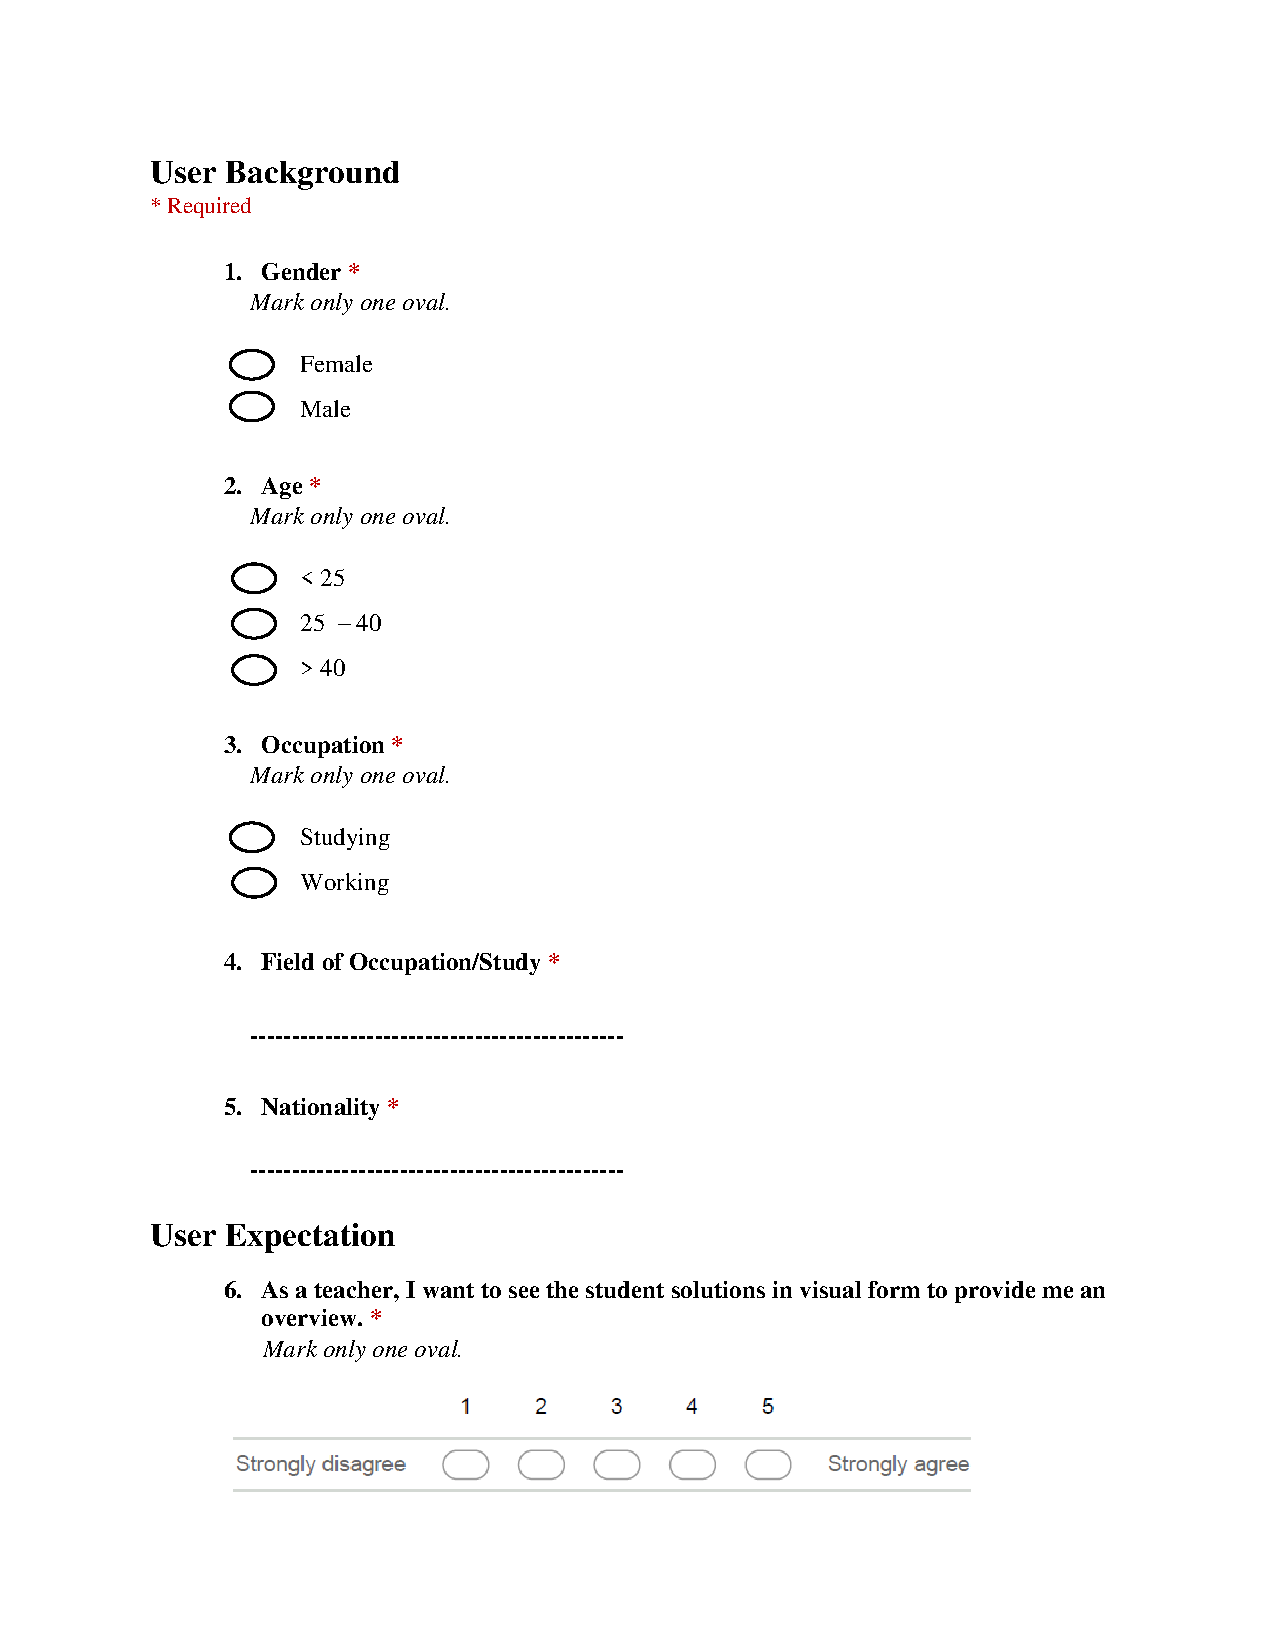
\includepdf[pages={1-}]{survey.pdf}


\end{appendices}

\end{document}
